\section{Background}

We usually experience the following steps when trying to get a well-focused photo:
\begin{enumerate}
	\item Get the image with the camera when the lens group is at the current position.
	\item Evaluate whether the image is blurred and get a value using the focus function.
	\item Compare the value with the previous value. If the value grows larger (image gets better focused), the current moving direction is correct.
	\item Move the lens group towards the direction.
	\item Repeat the process until the value gets smaller or the evaluated value cannot be further improved.
\end{enumerate}

During this process, we need to decide the focusing method we use, the focus function, how we move the lens group and the specifications of the camera we use.
Now we introduce the parts one by one.

\subsection{Existing Focusing Methods}
There are mainly three categories of focusing methods in current phones~\cite{autofocus}.

\textbf{Contrast Detection} is the standard and traditional method we use in most phones.
It applies trial and error.
The lens group move back and forth until the position of the maimum focus function value is found.
This method is slow and takes time to move the lens and evaluate the autofocus effects.
However, the outcome figures are fairly good in most cases, except for low-light conditions.

\begin{figure}[tb!]
	\begin{center}
		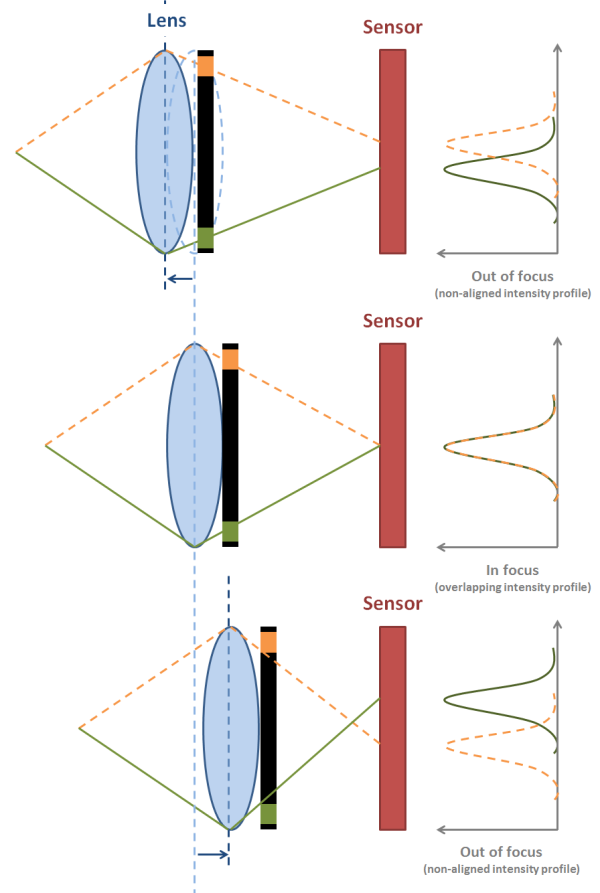
\includegraphics[width=2in]{phasedetection}
	\end{center}
	\caption{Basic ideas of phase detection}
	\label{f:phasedetection}
\end{figure}

\textbf{Phase Detection} is a better method which requires more expensive hardware.
This technique is usually applied in digital single-lens reflex cameras.
As shown in Figure~\ref{f:phasedetection}, there are 2 apertures on opposite sides of the lens and they leave 2 light rays which provides different intensity profile if they are not well focused.
The system can thus decide exactly how much the lens need to be adjusted according to the profiles.
This is much faster but requires better hardware and still suffers in low-light conditions.

\textbf{Laser detection} is a method similar to Radar and calculates the time for the laser to be reflected.
It is super fast and works in low-light conditions as well.
However, it is effective only in short distances and may be biased by transparent objects like windows.

\subsection{Focus Functions}

Focus functions are methods to evaluate whether a picture is well-focused.
In general, the functions include calculating sharpness difference with neighboring points for some sampling pixels or all pixels in the picture.

There are quite some papers explaining different focus functions~\cite{focusfunction}.
In general, there are 4 types based on derivatives, statistics, histograms and intuitive.
Statistics-based methods use variance or correlation of all the pixels.
Hisograms-based methods summarize the histogram of grey-level intensities of pixels and calculates the range or entopy.
Intuitive-based methods sums up the intensities above the threshold as the function.
These 3 types of methods above are less popular than derivative-based methods.
Here the derivative could be absolute difference, square, Laplacian operator, Sobel operator, etc.
Different methods have slightly different effect for various scenarios.

In our implementation, we use existing Python library and applies Laplacian operator.

\subsection{Hill Climbing}

Hill climbing is basicly trial-and-error.
We usually have a function $y=F(x)$ and a range for $x$.
We hope to find the maximum value of $y$ among the range of $x$.

$x$ starts from one edge of the range, select a basic step, and keep moving towards the other end at the interval of the step.
Every time when $x$ changes, we calculate the $y$ value and if $y$ increases, we keep move $x$ towards the same direction.
Otherwise, we reduce the step size and move $x$ towards the opposite direction.
This keeps going until the $y$ value cannot be further increased.

\begin{figure}[tb!]
	\begin{center}
		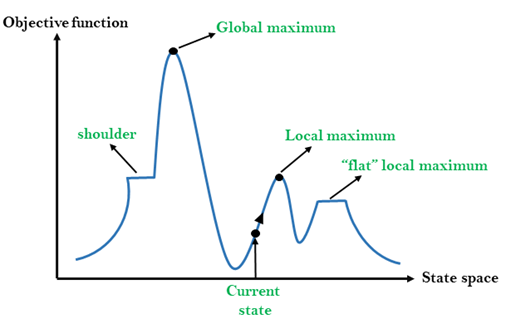
\includegraphics[width=2in]{hillclimb}
	\end{center}
	\caption{Example of traditional hill climbing}
	\label{f:hillclimb}
\end{figure}

As shown in Figure~\ref{f:hillclimb}, we can see that there are 1 global maximum and multiple local maximum.
Only using the method mentioned above, we may fall into local maximum and not get the best value.
Simulated annealing and random walks may help with the situation and lead us to global maximum.

\subsection{Camera Specifications}

\begin{figure}[tb!]
	\begin{center}
		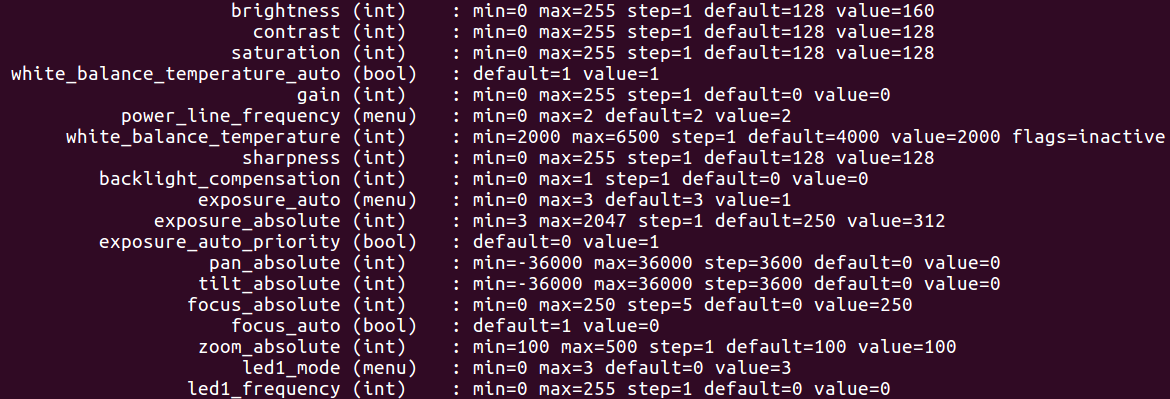
\includegraphics[width=3in]{param}
	\end{center}
	\caption{Controllable camera parameters}
	\label{f:param}
\end{figure}

We use Logitech C920 for the experiments.
This is a camera which follows UVC (USB video device class standard) and it can be controlled by v4l2 tool.
All the available parameters are listed in Figure~\ref{f:param}.

Among all the parameters, we care about focus\_absolute the most.
focus\_absolute ranges from 0 to 250 and the minimum step is 5.
The values are in millimeters, marking the position of the lens group in the camera.
This value can only be changed if we disable auto focus, which means setting focus\_auto to 0.
To be more clear, if the object distance if further, focus\_absolute needs to be larger, vice versa.

White balance temperature and Exposure time need to be changed as well.
white\_balance\_temperature\_auto needs to be 0 so that it is disabled.
The default temperature is 3000 but in my experiment environment it is better to be 4000.
exposure\_auto need to be 1, while 3 is full auto and 1 is completely manual.
exposure\_absolute has the default value of 250 and we set it 333 for better result contrast.
These 2 factors greatly impact the photo capturing time, which is a huge part of the overall time.

